\chapter{Supplementary Material and Output Results}
\label{ch:appendix}

This appendix provides supplementary materials, including United Nations Sustainable Development Goals (SDGs) alignment and the complete visual outputs generated during the experimental execution of the project.

\section{Alignment with UN Sustainable Development Goals (SDGs)}
\label{sec:sdg_alignment}

The methodologies and applications investigated in this project align directly with multiple United Nations Sustainable Development Goals (SDGs), as summarized in Table \ref{tab:sdg_mapping}.

\begin{table}[H]
\centering
\caption{United Nations Sustainable Development Goals Addressed by the Project}
\label{tab:sdg_mapping}
\begin{tabular}{p{2.5cm} p{3.5cm} p{8cm}}
\toprule
\textbf{SDG Number} & \textbf{Goal Title} & \textbf{Direct Relevance and Project Contribution} \\
\midrule
\textbf{SDG 15} & Life on Land & Promotes accurate, robust, and reproducible ecological classification models for forest inventory, species preservation, and sustainable management of terrestrial ecosystems. \\
\midrule
\textbf{SDG 9} & Industry, Innovation, and Infrastructure & Fosters scientific innovation and sound machine learning infrastructure by establishing verifiable protocols for experimental stability and reproducibility. \\
\midrule
\textbf{SDG 13} & Climate Action & Accurate forest cover type mapping supports long-term ecological monitoring and carbon sequestration tracking, assisting climate impact assessment. \\
\midrule
\textbf{SDG 4} & Quality Education & Demonstrates rigorous scientific methodologies, seed governance, and error quantification, providing educational value for future AI researchers and practitioners. \\
\bottomrule
\end{tabular}
\end{table}

\clearpage
\section{Output Screenshots and Visual Results}
\label{sec:output_results}

This section documents all primary graphical visualizations generated from the Jupyter Notebook execution, illustrating the exploratory data analysis, data distributions, and experimental benchmark comparisons.

\subsection{Exploratory Data Analysis Visualizations}

\begin{figure}[H]
\centering
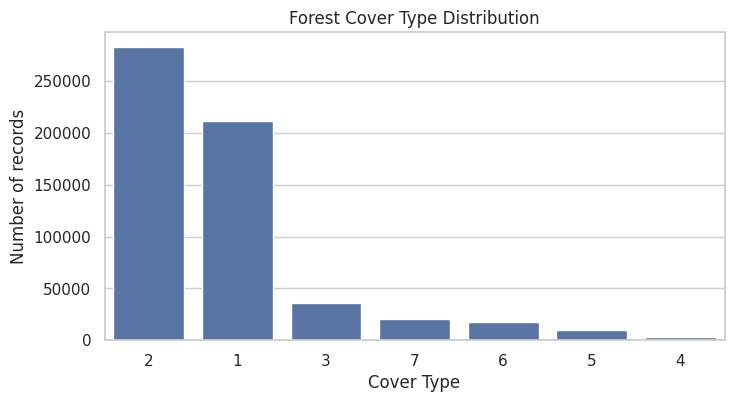
\includegraphics[width=0.88\textwidth]{figures/fig_class_distribution.png}
\caption{Forest CoverType Target Class Frequency Distribution (Showing High Imbalance)}
\label{fig:out_class_dist}
\end{figure}

\begin{figure}[H]
\centering
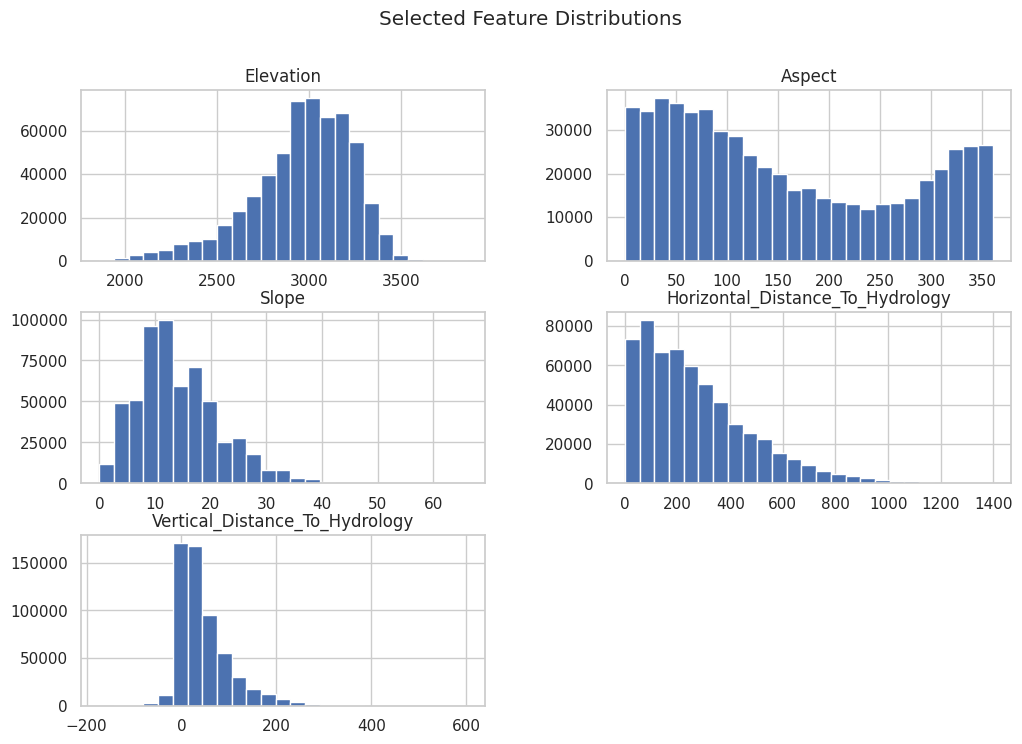
\includegraphics[width=0.92\textwidth]{figures/fig_continuous_features.png}
\caption{Distribution Histograms for 10 Continuous Cartographic Features}
\label{fig:out_histograms}
\end{figure}

\clearpage
\begin{figure}[H]
\centering
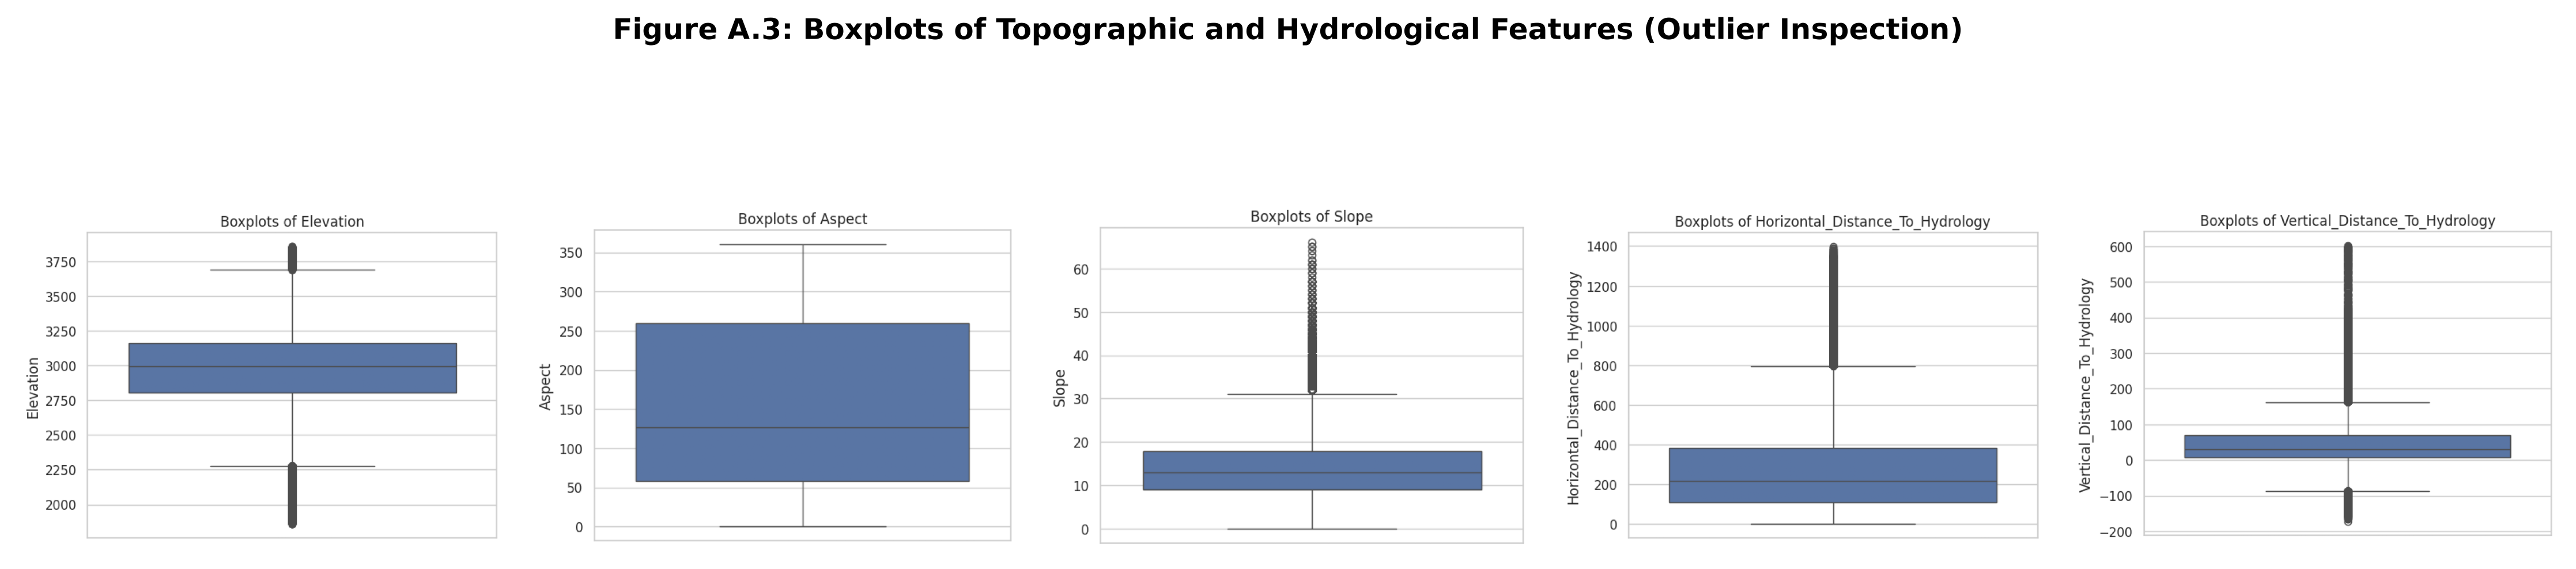
\includegraphics[width=0.92\textwidth]{figures/fig_boxplots.png}
\caption{Boxplots for Continuous Variables Illustrating Spread, Skewness, and Outliers}
\label{fig:out_boxplots}
\end{figure}

\begin{figure}[H]
\centering
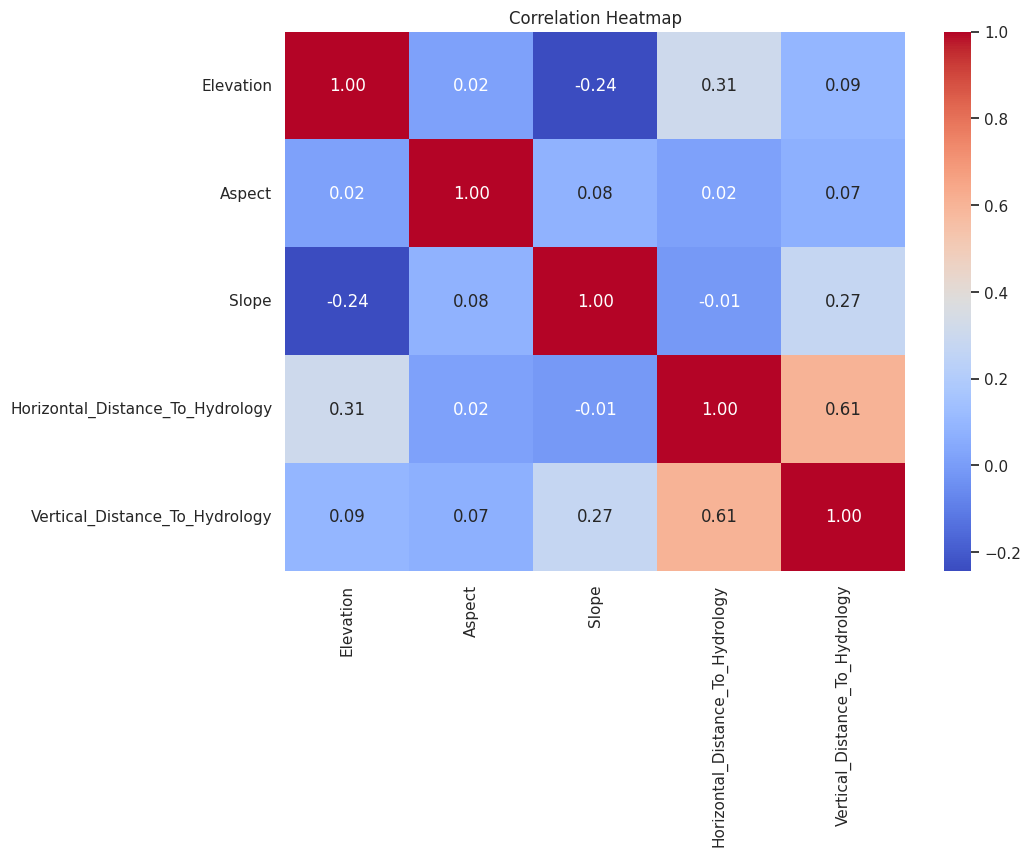
\includegraphics[width=0.85\textwidth]{figures/fig_correlation_matrix.png}
\caption{Correlation Heatmap of Continuous Cartographic Variables}
\label{fig:out_correlation}
\end{figure}

\clearpage
\subsection{Experimental Results and Comparative Evaluation}

\begin{figure}[H]
\centering
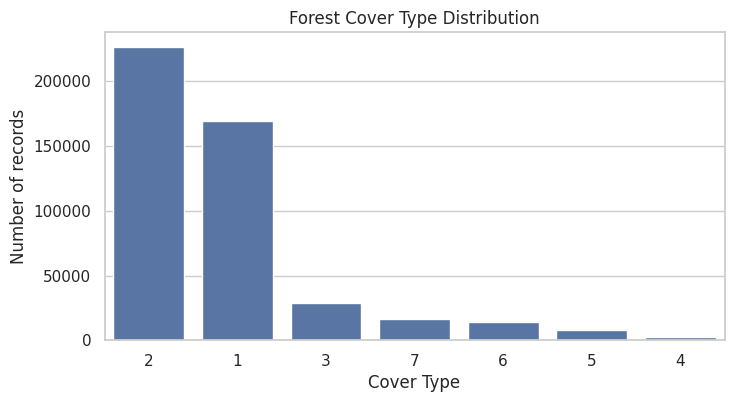
\includegraphics[width=0.85\textwidth]{figures/fig_train_test_split.png}
\caption{Stratified Train-Test Split Class Distribution Verification ($80/20$ Partition)}
\label{fig:out_train_split}
\end{figure}

\begin{figure}[H]
\centering
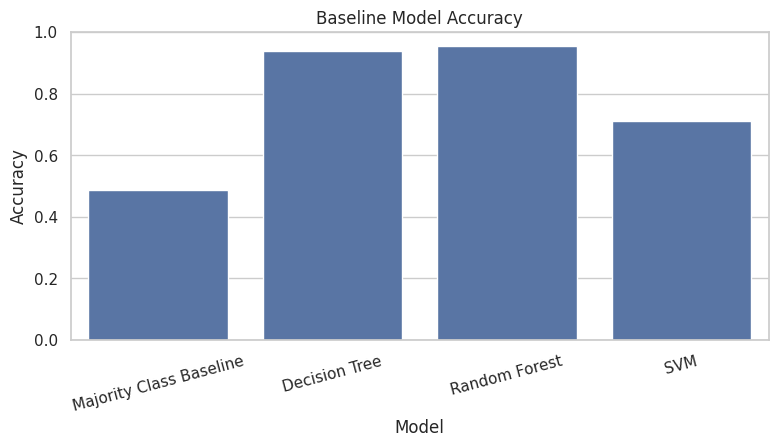
\includegraphics[width=0.85\textwidth]{figures/fig_baseline_accuracy.png}
\caption{Baseline Classification Accuracy Comparison Across Algorithms (Seed 42)}
\label{fig:out_baseline_acc}
\end{figure}

\clearpage
\begin{figure}[H]
\centering
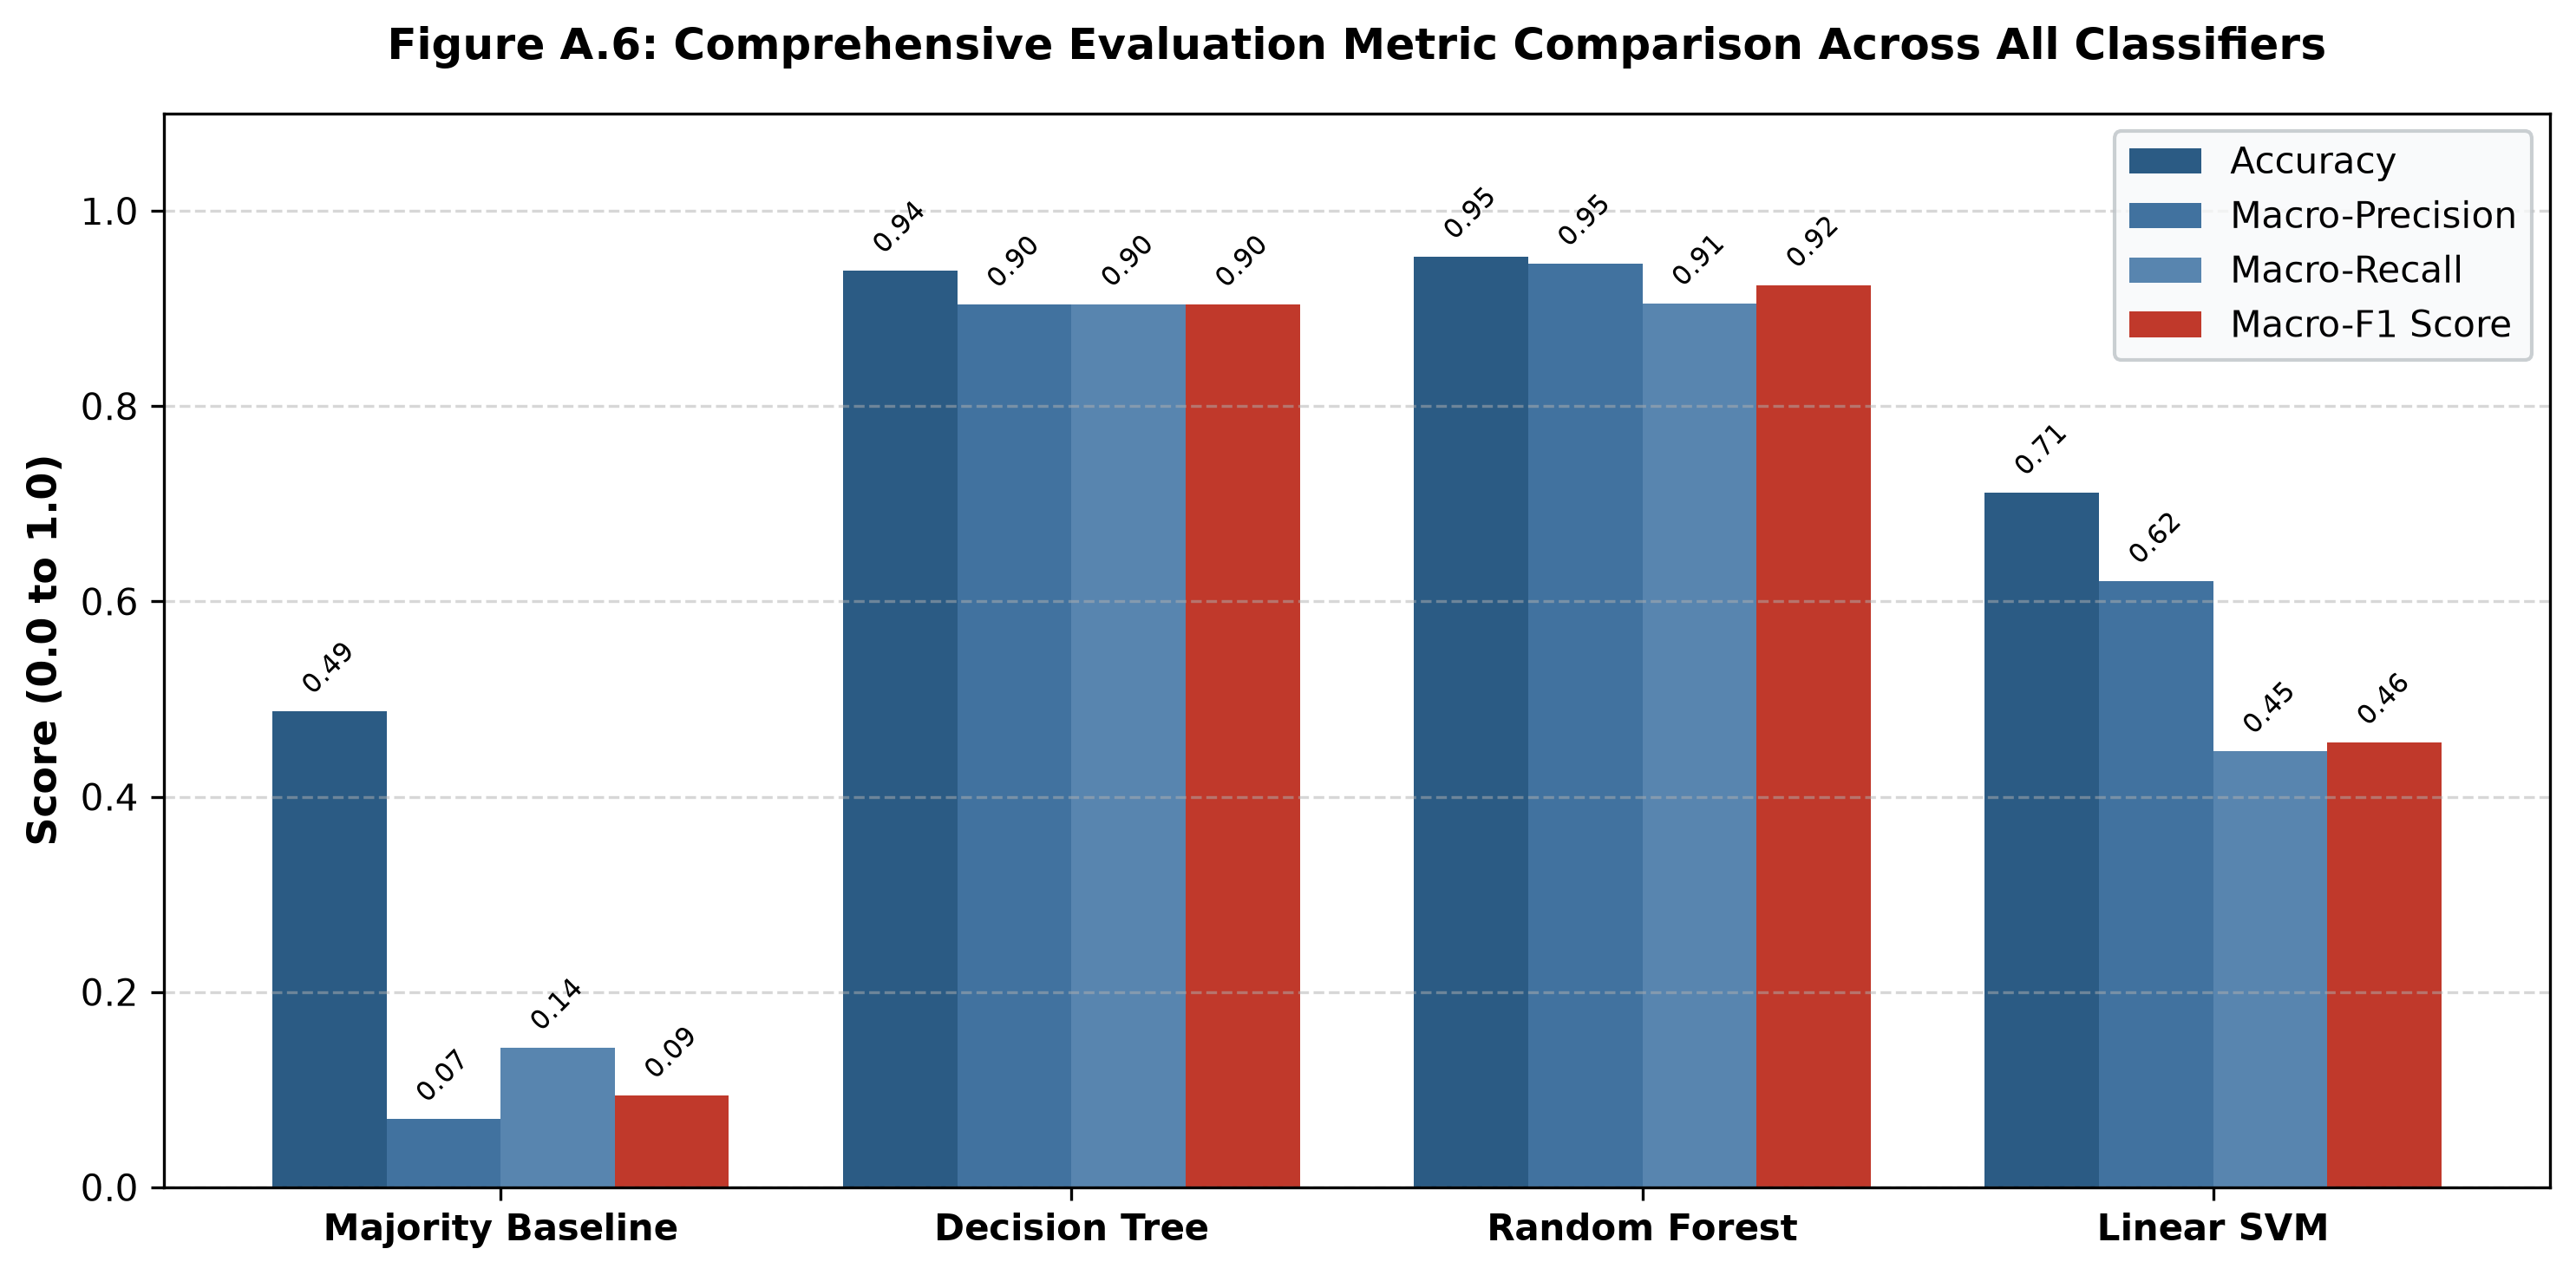
\includegraphics[width=0.88\textwidth]{figures/fig_metric_comparison.png}
\caption{Comprehensive Performance Metrics (Accuracy, Precision, Recall, Macro-F1)}
\label{fig:out_metric_comp}
\end{figure}

\begin{figure}[H]
\centering
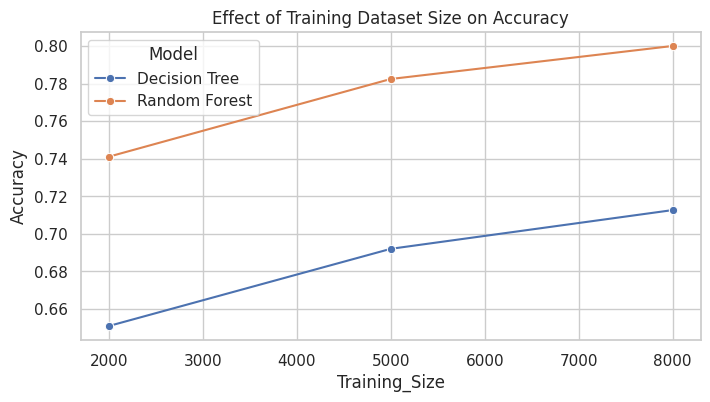
\includegraphics[width=0.85\textwidth]{figures/fig_data_scaling.png}
\caption{Model Accuracy Trajectory Across Increasing Subsample Sizes ($N=1,000$ to $10,000$)}
\label{fig:out_scaling}
\end{figure}
